\documentclass[12pt, a4paper]{article}
\usepackage{cmap} % Улучшенный поиск русских слов в полученном pdf-файле
\usepackage[T2A]{fontenc} % Поддержка русских букв
\usepackage[utf8]{inputenc} % Кодировка utf8
\usepackage[english,russian]{babel} % Языки: русский, английский
%\usepackage{pscyr} % Нормальные шрифты
\usepackage{amsmath}
\usepackage{geometry}

\geometry{left=30mm}
\geometry{right=10mm}
\geometry{top=20mm}
\geometry{bottom=20mm}

\usepackage{titlesec}
\titleformat{\section}
{\normalsize\bfseries}
{\thesection}
{1em}{}
\titlespacing*{\chapter}{0pt}{-30pt}{8pt}
\titlespacing*{\section}{\parindent}{*4}{*4}
\titlespacing*{\subsection}{\parindent}{*4}{*4}
\titlespacing*{\subsubsection}{\parindent}{*4}{*4}
\usepackage{setspace}
\onehalfspacing % Полуторный интервал
\frenchspacing
\usepackage{indentfirst} % Красная строка
\usepackage{titlesec}
\titleformat{\chapter}{\LARGE\bfseries}{\thechapter}{20pt}{\LARGE\bfseries}
\titleformat{\section}{\Large\bfseries}{\thesection}{20pt}{\Large\bfseries}
\usepackage{listings}
\usepackage{xcolor}

%%% Insert pdf pages
\usepackage[final]{pdfpages}
\usepackage{pgfplots}
\usetikzlibrary{datavisualization}
\usetikzlibrary{datavisualization.formats.functions}
\usepackage{graphicx}

\newcommand{\img}[3] {
    \begin{figure}[!ht]
        \center{\includegraphics[height=#1]{assets/img/#2}}
        \caption{#3}
        \label{img:#2}
    \end{figure}
}

%Подписи
\usepackage		[margin		= 10	pt,
%					font		= footnotesize, 
%labelfont	= bf, 
labelsep	= endash, 
%labelfont	= bf,
%					textfont	= sl,
margin		= 0 	pt,  
aboveskip 	= 4		pt, 
belowskip 	= -6	pt,
figurename= Рисунок] {caption}

\makeatletter
\renewcommand{\thefigure}{\thesection.\@arabic\c@figure}
\renewcommand{\thetable}{\thesection.\@arabic\c@table}
\makeatother

\makeatletter % список литературы
\def\@biblabel#1{#1. }
\makeatother


\usepackage[justification=centering]{caption} % Настройка подписей float объектов
\usepackage[unicode,pdftex]{hyperref} % Ссылки в pdf
\hypersetup{hidelinks}
\newcommand{\code}[1]{\texttt{#1}}
\usepackage{icomma} % Интеллектуальные запятые для десятичных чисел
\usepackage{csvsimple}

% Для листинга кода:
\lstset{ %
	language=c++,                 % выбор языка для подсветки (здесь это С++)
	basicstyle=\small\sffamily, % размер и начертание шрифта для подсветки кода
	numbers=left,               % где поставить нумерацию строк (слева\справа)
	numberstyle=\tiny,           % размер шрифта для номеров строк
	stepnumber=1,                   % размер шага между двумя номерами строк
	numbersep=5pt,                % как далеко отстоят номера строк от подсвечиваемого кода
	showspaces=false,            % показывать или нет пробелы специальными отступами
	showstringspaces=false,      % показывать или нет пробелы в строках
	showtabs=false,             % показывать или нет табуляцию в строках
	frame=single,              % рисовать рамку вокруг кода
	tabsize=2,                 % размер табуляции по умолчанию равен 2 пробелам
	captionpos=t,              % позиция заголовка вверху [t] или внизу [b] 
	breaklines=true,           % автоматически переносить строки (да\нет)
	breakatwhitespace=false, % переносить строки только если есть пробел
	escapeinside={\#*}{*)}   % если нужно добавить комментарии в коде
}

\begin{document}
%	\counterwithin{lstlisting}{section}
%	\includepdf[pages=-]{titlesheet.pdf}
	
\includepdf[pages=1]{title.pdf}
	
\includepdf[pages=1]{task.pdf}
	
\includepdf[pages=1]{review.pdf}
	
%	\setcounter{page}{3}
	
%	\input{00-essay.tex}
%	\newpage
	
	% Содержание
	\tableofcontents
	\newpage
	
%	\printnomenclature[2em]
%	В тексте писать так: $\beta$\nomenclature{$\beta$}{Вторая буква греческого алфавита}
	
	\section*{Введение}
\addcontentsline{toc}{section}{Введение}

\textbf{Головка самонаведения} (ГСН) — автоматическое устройство, которое устанавливается на управляемое средство поражения (ракету, бомбу, торпеду и др.) для обеспечения прямого попадания в объект атаки или сближение на расстояние, меньшее радиуса поражения боевой части средства поражения (СП), то есть для обеспечения высокой точности наведения на цель. ГСН является элементом системы самонаведения. \cite{book1} \\

СП, оборудованное ГСН, может «видеть» «подсвеченную» носителем или ей самой, излучающую или контрастную цель и самостоятельно наводиться на неё, в отличие от ракет, наводимых командным способом. \\

Виды ГСН:
\begin{itemize}
	\item \textbf{РГС (РГС, РЛГСН) — радиолокационная ГСН};
	\item ТГС (ИКГСН) — тепловая, инфракрасная ГСН;
	\item ТВГСН — телевизионная ГС;
	\item ТПВГС - тепловизионная ГС;
	\item ЛГСН - Лазерная ГС.
\end{itemize}

Канал межблочного обмена (КМБО) может быть использован для обмена данными между управляющей ЭВМ и внешними устройствами (в частности, НЧ и СВЧ аппаратурой) в режиме реального времени. Техническим результатом является повышение точности синхронизации обмена данными. \cite{book2} \\

\textbf{Цель} работы - разработать и отладить библиотеку алгоритмов взаимодействия персонального компьютера (ПК) и контрольной измерительной аппаратурой радиолокационной головкой самонаведения (КИА РГС). \\

Выделены следующие \textbf{задачи}:
\begin{enumerate}
	\item[1)] ознакомиться с алгоритмами взаимодействия ПК и КИА РГС;
	\item[2)] изучить протокол канала межблочного обмена (КМБО);
	\item[3)] проработать особенности работы с PCI, USB, Ethernet;
	\item[4)] разработать соответствующую библиотеку алгоритмов и отладить её.
\end{enumerate}
	\newpage
	
	\section*{Основная часть}
\addcontentsline{toc}{section}{Основная часть}
\section{Общие положения}
	\subsection{Канал межблочного обмена (КМБО)}
		\subsubsection{Основные характеристики канала}
		Скорость передачи данных - 1000 Кбит/сек.\\
		
		Расстояние передачи – до 10 м.
		
		\subsubsection{Состав канала}
		В состав канала обмена входят:
		\begin{itemize}
			\item ведущая станция – ПК с контроллером;
			\item оконечные устройства – модули блоков аппаратуры. \\
		\end{itemize}
	
		При необходимости к каналу может подключаться вспомогательное (сервисное) оборудование на правах оконечных устройств.
		Общее количество устройств в составе канала:
		\begin{itemize}
			\item контроллер – 1;
			\item оконечные устройства – до 32. \\
		\end{itemize}
	
		Ведущей станцией, управляющей обменом, является \textbf{контроллер}. \textbf{Оконечные устройства} осуществляют прием информации от контроллера или передачу информации контроллеру под управлением контроллера. \\
		
		Для организации линии связи между контроллером и оконечными устройствами используются две двухпроводные магистральные линии:
		\begin{itemize}
			\item линия передачи тактового сигнала (SYN); 
			\item линия передачи данных (DATA). \\
		\end{itemize}	
	
		Взаимный обмен информацией между контроллером и оконечными устройствами осуществляется \textbf{кадрами информации}.
		
		\subsubsection{Форматы кадров информационного обмена}
		Форматы кадров разделяется на два вида:
		\begin{itemize}
			\item формат кадра передачи информации от контроллера (кадр W);
			\item формат кадра приема информации от оконечного устройства (кадр R). \\
		\end{itemize}
		
		\textbf{Формат кадров} W и R одинаковый и имеет вид: \\
		
		\begin{tabular}{ | c | c | c | c | c| c | }
			\hline
			ЗАГ & ИС & ИС & ... & ИС & БЧ \\
			\hline
		\end{tabular}
		\\
		
		где:
		
		\qquad ЗАГ – заголовок кадра (16 бит);
		
		\qquad ИС – информационное слово (16 бит). Количество информационных слов в кадре – от одного до 64;
		
		\qquad БЧ – бит четности (1 бит). \\
		
		При формировании кадров W на линии данных контроллер является активным на протяжении всего кадра. По окончании кадра контроллер переводится в состояние паузы.\\
		
		При формировании кадров R на линии данных контроллер является активным на протяжении заголовка кадра. По окончании заголовка контроллер переводится в состояние паузы. На протяжении части кадра, соответствующей ИС и БЧ, на линии данных активным является оконечное устройство. \\
		
		По линии тактового сигнала контроллер является активным как во время кадра (W или R), так и в паузе между кадрами. Оконечные устройства по линии тактового сигнала работают только на прием. \\
		
		\textbf{Формат заголовка кадра} имеет вид: \\
		
		\begin{tabular}{ | c | c | c | c | }
			\hline
			АДР & W/R & ЧС & БЗЧ \\
			\hline
		\end{tabular}
		\\
		
		где:
		
		\qquad АДР –  адрес оконечного устройства (8 бит);
		
		\qquad W/R – признак Передача - Чтение (1 бит);
		
		\qquad ЧС   – число информационных слов в кадре (6 бит);
		
		\qquad БЧЗ  – бит четности заголовка (1 бит). \\
		
		\textbf{Адрес оконечного устройства} – положительное двоичное число от 1 до 255. Передача адреса начинается со старшего разряда и кончается младшим разрядом. \\
		
		\textbf{Признак W/R} – 1 бит, имеет значение 0 – передача данных от контроллера оконечному устройству (кадр W), 1 – прием данных от оконечного устройства (кадр R). \\
		
		\textbf{Число информационных слов} в кадре – положительное двоичное число от 1 до 64. Передача ЧС начинается со старшего разряда и кончается младшим разрядом. Код 000000 соответствует числу слов 64. \\
		
		\textbf{Бит четности заголовка} дополняет заголовок до нечетности. \cite{kmbo}\\
		
		Числовая информация передается дополнительным кодом.\\
		
		\subsubsection{Требования к контроллеру}
		Контроллер, как правило, является устройством, управляемым программно процессором ПК. 
		Может находиться в двух состояниях:
		\begin{itemize}
		\item состояние паузы;
		\item состояние работы.
		\end{itemize}
		
		В \textbf{состоянии паузы} контроллер находится в перерыве между кадрами передачи или приема информации. \\
		
		В \textbf{состоянии работы} контроллер осуществляет прием или передачу заданного числа слов. \\
		
		\textbf{При передаче данных (кадр W)} контроллер передает заголовок, заданное число слов и бит четности БЧ. Бит четности вычисляется контроллером аппаратно. После окончания передачи кадра контроллер переходит в состояние паузы. \\
		
		\textbf{При приеме данных (кадр R)} контроллер передает заголовок, после чего принимает заданное число слов и бит четности БЧ. Проверка соответствия бита четности проводится контроллером аппаратно. После окончания приема кадра контроллер переходит в состояние паузы. \\
		
		\textbf{При передаче кадра W}, а также при передаче заголовка кадра R контроллер одновременно производит чтение с линии данных, которые он сам передал, и аппаратно производит сравнение переданных и принятых данных. Результат (1 бит,  0 - при совпадении, 1 - при несовпадении) должен быть доступен для чтения процессору по окончании кадра.
		
		\subsubsection{Требования к оконечному устройству}
		Оконечное устройство, как правило, является аппаратным устройством и функционирует в соответствии с заложенным в него алгоритмом. При этом оконечное устройство может находиться в 4-х состояниях:
		\begin{itemize}
			\item  исходное состояние;
			\item  состояние приема заголовка кадра;
			\item  состояние ожидания паузы;
			\item  состояние работы. \\
		\end{itemize}
	
		После приема заголовка кадра (16 бит) устройство сравнивает адрес АДР в заголовке с собственным адресом.\\
		
		При совпадении адреса и правильном бите четности заголовка БЧЗ оконечное устройство переходит в состояние работы. При этом в зависимости от бита W/R осуществляется прием данных с линии или выдача данных на линию. Устройство принимает или передает число слов, на которое оно настроено аппаратно. По окончании приема или передачи указанного числа слов и бита четности БЧ устройство переходит в состояние ожидания паузы. \\
		
		Характер исполнения принятой устройством информации при несовпадении числа слов в кадре и аппаратно заложенного в устройство числа слов, а также при неправильном бите четности кадра БЧ настоящим протоколом не определяется и устанавливается в каждом случае отдельно. \\
		
		При несовпадении адреса или неправильном бите четности заголовка БЧЗ оконечное устройство переходит в состояние ожидания паузы.
		
	\subsection{USB-КМБО}
	\subsubsection{Общее}
	Контроллер реализован в виде внешнего USB модуля с размерами 30мм $\times$ 85мм $\times$ 145мм и предназначен для сопряжения персонального компьютера (ПК) через порт USB с каналом межблочного обмена (КМБО) и каналами разовых (битовых) команд (РК) и используется в составе автоматизированной контрольно-испытательной аппаратуры (АКИА). \\
	
	В отличие от контроллера PCI-КМБО контроллер USB-КМБО имеет ряд дополнительных функций, позволяющих производить проверку работы аппаратуры при предельных отклонениях временных параметров сигналов КМБО. \\
	
	Контроллер включает в себя ПЛИС (программируемая логическая интегральная схема), реализующую протокол обмена КМБО, приемо-передатчики сигналов КМБО и интерфейсное устройство шины USB (микросхема FT2232H). \cite{FT2232H} \\
	
	FTDI – драйвер и библиотека функций микросхемы FT2232H, используемой в контроллере USB-КМБО. \cite{ftdi}
	
	\subsubsection{Состав изделия}
	В состав изделия входят следующие функциональные узлы.
	\begin{enumerate}
		\item \textbf{ППЗУ} - перепрограммируемое постоянное запоминающее устройство (EEPROM), предназначено для хранения данных конфигурации изделия.
		\item \textbf{Интерфейс ППЗУ} обеспечивает чтение ППЗУ и его программирование по шине USB.
		\item \textbf{Интерфейс USB} обеспечивает протокол обмена изделия с шиной USB.
		\item \textbf{Кварцевый генератор с умножителем} обеспечивает формирование тактовых импульсов с частотами 6, 12 и 48 МГц.
		\item \textbf{Приемный буфер RX} предназначен для приема информации, поступающей с шины USB, с последующей передачей ее в узлы микросхемы EPM9320LC84.
		\item \textbf{Передающий буфер TX} предназначен для передачи информации в шину USB, поступающей от узлов микросхемы EPM9320LC84.
		\item \textbf{Регистр выходных РК} обеспечивает прием и хранение разовых команд РК, поступающих с шины USB в приемный буфер RX.
		\item \textbf{Регистр командного слова} обеспечивает прием и дешифрацию командного слова, поступающего с шины USB в приемный буфер RX.
		\item \textbf{Интерфейс КМБО} обеспечивает формирование W-кадров и заголовков R-кадров информации КМБО, значения которых считываются из приемного буфера RX, а также прием данных R-кадров и запись их в передающий буфер TX. Устройство осуществляет также формирование бита четности в кадрах W, контроль бита четности в кадрах W и R (ВН) и т.д.
		\item \textbf{Регистр входных РК} обеспечивает передачу входных разовых команд РК в передающий буфер TX.
		\item \textbf{Твердотельные реле} предназначены для выдачи выходных РК.
		\item \textbf{Приемопередатчики RS-485} обеспечивают формирование уровней сигналов КМБО.
	\end{enumerate}

	\subsection{PCI-КМБО}
	\subsubsection{Основные части}
	Изделие состоит из следующих функциональных устройств.
	\begin{enumerate}
		\item \textbf{Интерфейс PCI} обеспечивает связь изделия с шиной PCI ПЭВМ. Обмен информацией между изделием и ПЭВМ осуществляется через четыре порта ввода/вывода и один канал прерывания.
		\item \textbf{Конфигурационная память} выполняет координационные функции по распределению ресурсов между устройствами при помощи специальной конфигурационной программы операционной системы ПЭВМ. После загрузки операционной системы в соответствующих регистрах конфигурационной памяти можно прочитать выделенные изделию базовый адрес ввода/вывода и номер канала прерывания.
		\item \textbf{Буферное запоминающее устройство (БЗУ)} обеспечивает хранение передаваемых и принимаемых данных КМБО. БЗУ двухпортовое, через первый порт происходит обмен информацией между БЗУ и ПЭВМ, через второй порт – между БЗУ и КМБО. Обмен между БЗУ и КМБО происходит во время передачи или приема кадров информации КМБО, а между БЗУ и ПЭВМ - в паузах между кадрами.
		\item\textbf{ Счетчик адреса} обеспечивает последовательные запись или чтение информации в/из БЗУ. 
		\item \textbf{Регистры}, предназначенные для управления изделием со стороны ПЭВМ.
		\item \textbf{Устройство синхронизации} обеспечивает синхронную работу составных узлов изделия и формирование структуры кадра.
		\item \textbf{Устройство формирования сигналов КМБО} обеспечивает формирование 
		W-кадров и заголовков R-кадров информации КМБО, значения которых хранятся в БЗУ, а также прием данных R-кадров и запись их в БЗУ. Устройство осуществляет также формирование бита четности в кадрах W, контроль бита четности в кадрах W и R (ВН) и контроль встречной работы (ВР).
		\item \textbf{Формирователь прерываний} обеспечивает формирование сигнала прерываний от таймера и по окончании передачи/приема кадров КМБО. 
		\item \textbf{Таймер} обеспечивает формирование импульсов с программируемым периодом следования. 
		\item \textbf{Счетчик времени}
	\end{enumerate}

	\subsubsection{Режимы изделия}
	Контроллер может находится в следующих режимах.
	\begin{enumerate}
		\item \textbf{Режим ВЫКЛ}\\
		В этом режиме через конфигурационные регистры производится проверка наличия подключенного изделия, чтение базового адреса и номера прерывания, назначенные операционной системой ПЭВМ (персональной электронной вычислительной машиной), и перевод изделия в режим ПОКОЙ.
		
		\item \textbf{Режим ПОКОЙ} \\
		Отличается от режима ВЫКЛ тем, что появляется возможность записи/чтения рабочих регистров изделия для установки режимов его работы. 
		
		\item \textbf{Режим КОНТРОЛЛЕР} \\
		Включается программно. В этом режиме изделие функционирует в режиме ведущей станции (контроллера) и обеспечивает следующие функции:
		\begin{itemize}
			\item обмен информацией по линии связи, скорость задается программно;
			\item хранение передаваемых и принимаемых данных в БЗУ (буферное запоминающее устройство) емкостью в 64 шестнадцатиразрядных слов;
			\item формирование кадров передачи данных (кадры W) и приема данных (кадры R) длиной от 1 до 64 информационных слов;
			\item аппаратное формирование бита четности в кадрах W и аппаратный контроль бита четности в кадрах W и R;
			\item аппаратное побитное сравнение передаваемых и принимаемых данных;
			\item формирование сигнала прерывания в конце каждого кадра.
		\end{itemize}
	\end{enumerate}

	\subsection{Ethernet-КМБО}
	\subsubsection{Общее}
	МС – устройство, сопрягающее персональный компьютер ПК, активный канал и канал радиокоррекции (РК). \\
	
	Применяется в составе аппаратуры контроля головки. Назначение модуля – преобразование интерфейсов КМБО и МКИО, контроль источников напряжения, выдача битовых команд. МС соединятся с ПК по Ethernet интерфейсу, с активным каналом по МКИО, с каналом РК по каналу межблочного обмена (КМБО). \cite{mc}
	
	\subsection{Вывод}
	Необходимо учесть все особенности работы с платами PCI-КМБО, USB-КМБО, Ethernet-КМБО для того, чтобы разработать необходимую библиотеку для информационного взаимодействия ПК и измерительной аппаратуры.
	
	
		
		
		
		
		

		
	\newpage
	
%	\setcounter{table}{0}
%	\setcounter{figure}{0}
	\newpage
\section{Конструкторский раздел}
В этом разделе будут подробно описаны основные функции библиотеки, приведены схемы их работы.

	\subsection{Общий алгоритм}
	Общий алгоритм выглядит следующим образом (рисунок \ref{fig1:image}):
	
	\begin{figure}[ph!]
		\centering
		\begin{center}
			{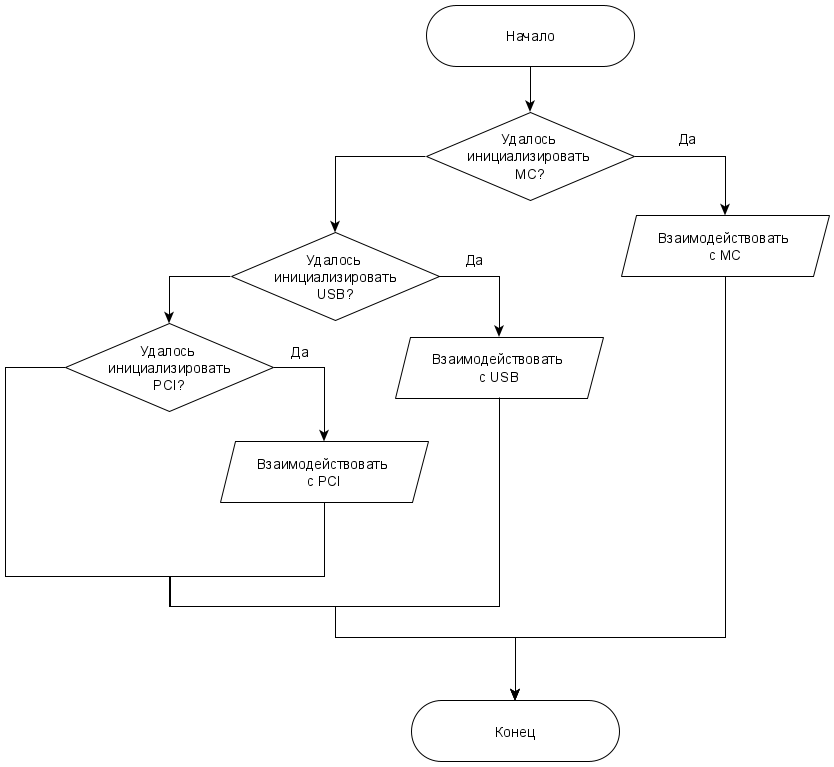
\includegraphics[scale=0.5]{schemes/general.png}}
			\caption{Общий алгоритм}
			\label{fig1:image}
		\end{center}
	\end{figure}


	\subsection{USB}
	\subsubsection{Функция инициализации (USB$\_$Open)}
	
	Схема изображена на рисунке \ref{fig2:image}.
	
	\begin{figure}[ph!]
		\centering
		\begin{center}
			{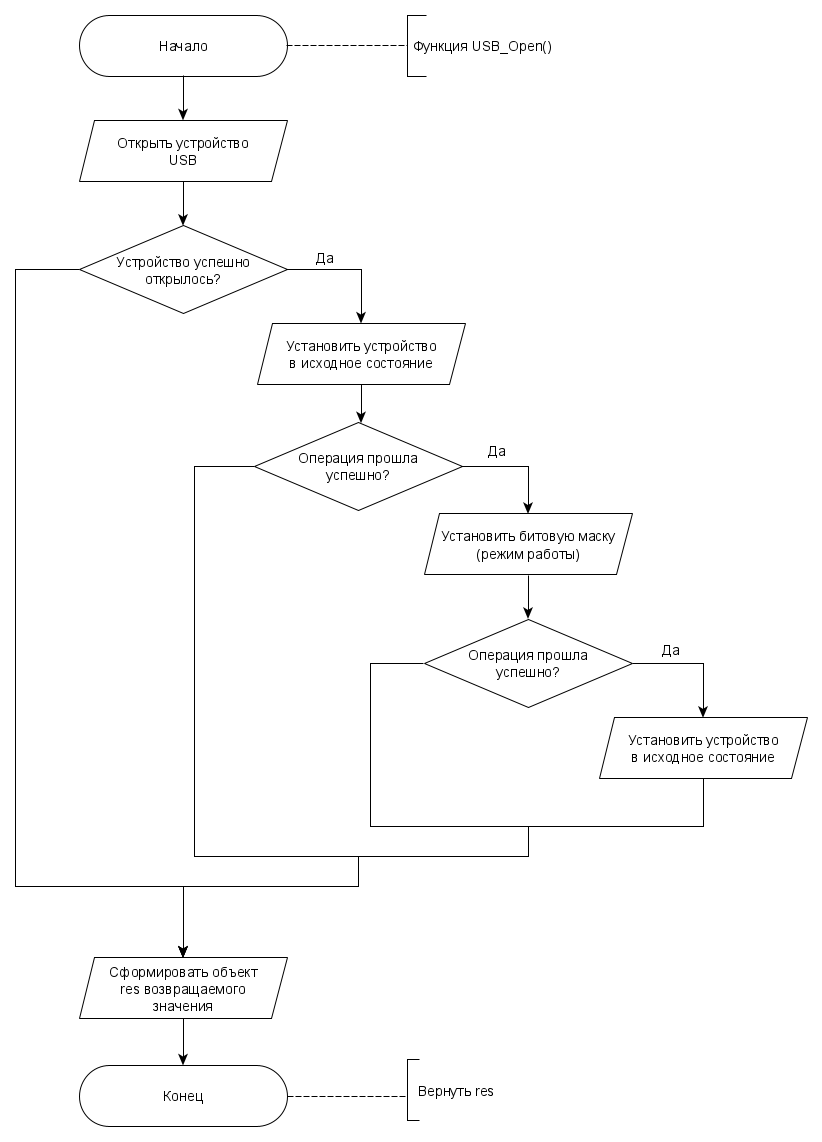
\includegraphics[scale=0.5]{schemes/usb_open.png}}
			\caption{USB$\_$Open()}
			\label{fig2:image}
		\end{center}
	\end{figure}

	\subsubsection{Прекращение работы с USB (USB$\_$Close)}
	
	Схема изображена на рисунке \ref{fig3:image}.
	
	\begin{figure}[ph!]
		\centering
		\begin{center}
			{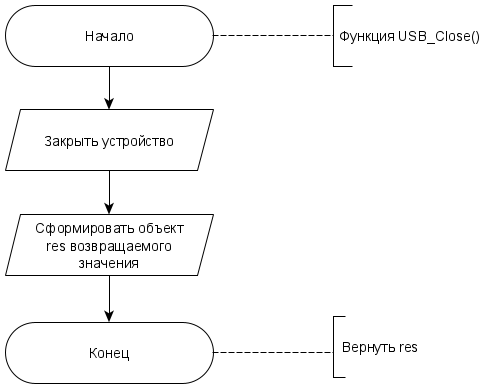
\includegraphics[scale=0.5]{schemes/usb_close.png}}
			\caption{USB$\_$Close()}
			\label{fig3:image}
		\end{center}
	\end{figure}

	\subsubsection{Функция записи данных в устройство USB-КМБО (USB$\_$Write)}

	Схема изображена на рисунке \ref{fig4:image}.
	
	\begin{figure}[ph!]
		\centering
		\begin{center}
			{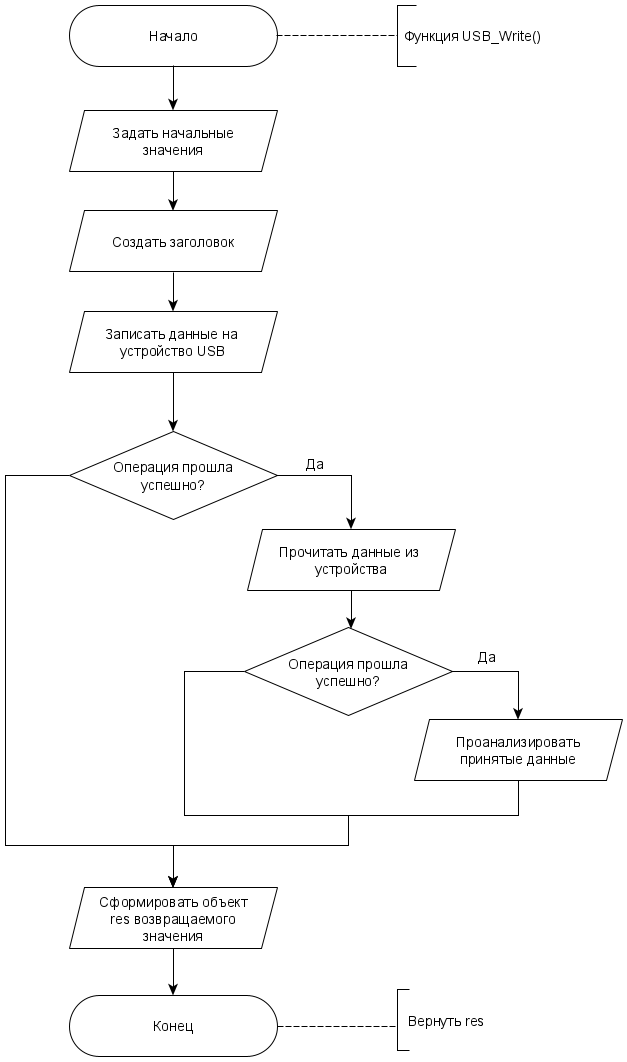
\includegraphics[scale=0.5]{schemes/usb_write.png}}
			\caption{USB$\_$Write()}
			\label{fig4:image}
		\end{center}
	\end{figure}

	\newpage

	\subsubsection{Функция чтения данных из устройства USB-КМБО (USB$\_$Read)}
	
	Схема изображена на рисунке \ref{fig5:image}.
	
	\begin{figure}[ph!]
		\centering
		\begin{center}
			{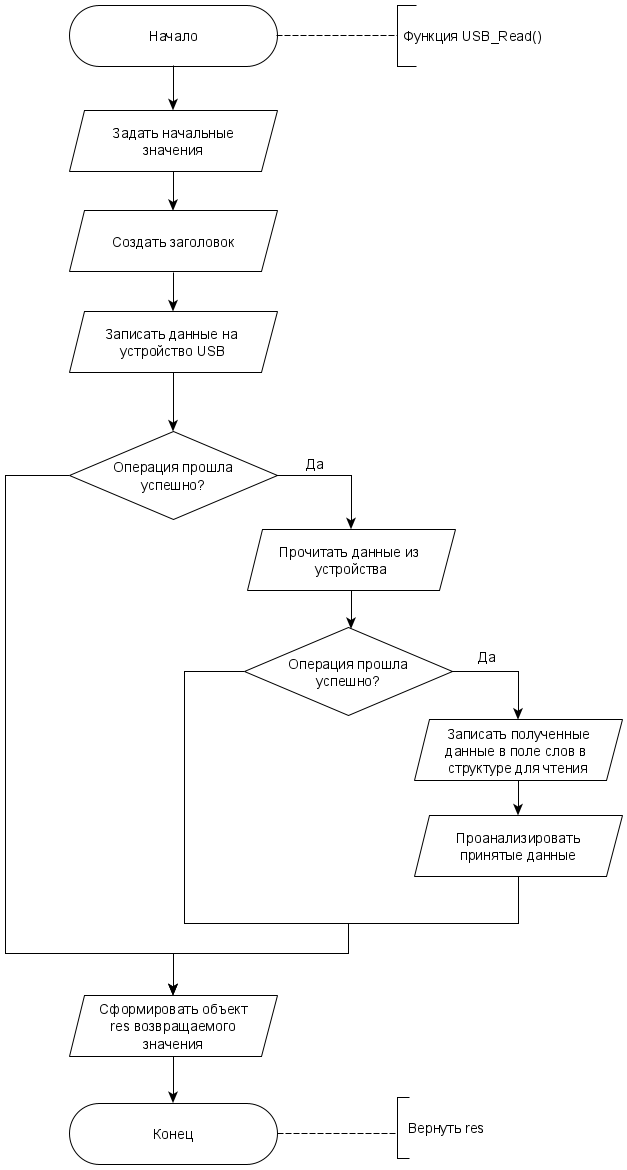
\includegraphics[scale=0.5]{schemes/usb_read.png}}
			\caption{USB$\_$Read()}
			\label{fig5:image}
		\end{center}
	\end{figure}

	\subsection{PCI}
	\subsubsection{Функция инициализации (PCI$\_$Open)}
	
	Схема изображена на рисунке \ref{fig6:image}.
	
	\begin{figure}[ph!]
		\centering
		\begin{center}
			{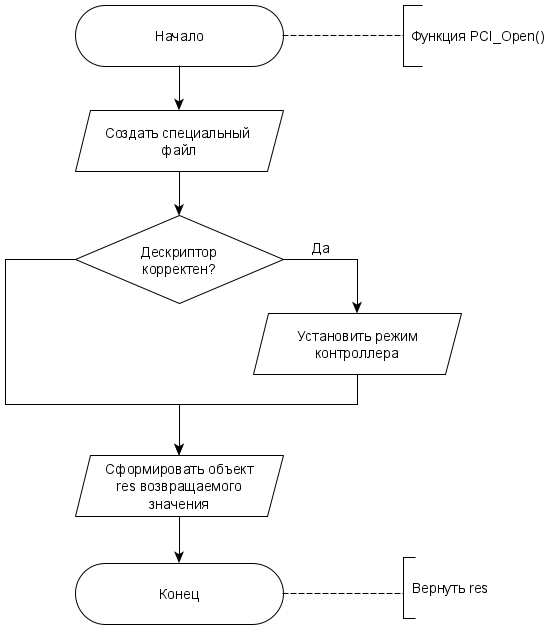
\includegraphics[scale=0.5]{schemes/pci_open.png}}
			\caption{PCI$\_$Open()}
			\label{fig6:image}
		\end{center}
	\end{figure}

	\newpage

	\subsubsection{Прекращение работы с PCI (PCI$\_$Close)}

	Схема изображена на рисунке \ref{fig7:image}.
	
	\begin{figure}[ph!]
		\centering
		\begin{center}
			{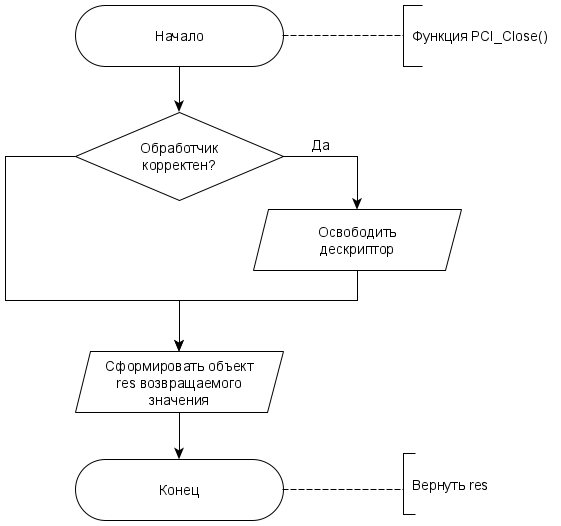
\includegraphics[scale=0.5]{schemes/pci_close.png}}
			\caption{PCI$\_$Close()}
			\label{fig7:image}
		\end{center}
	\end{figure}

	\newpage
	\subsubsection{Функция записи данных в устройство PCI-КМБО (PCI$\_$Write)}

	Схема изображена на рисунке \ref{fig8:image}.
	
	\begin{figure}[ph!]
		\centering
		\begin{center}
			{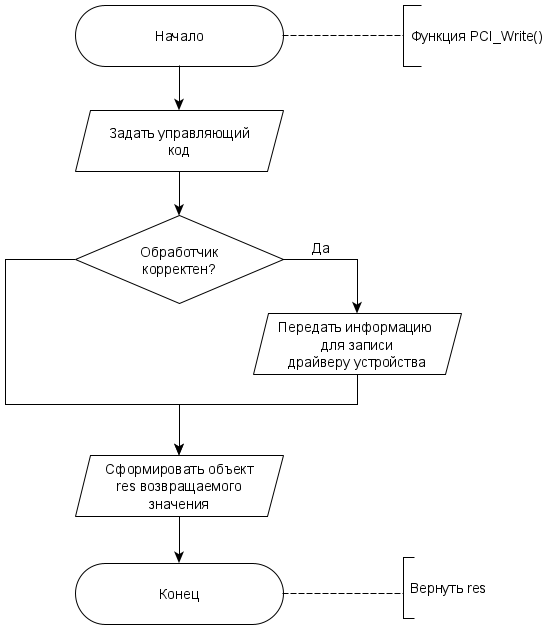
\includegraphics[scale=0.5]{schemes/pci_write.png}}
			\caption{PCI$\_$Write()}
			\label{fig8:image}
		\end{center}
	\end{figure}

	\newpage
	
	\subsubsection{Функция чтения данных из устройства PCI-КМБО (PCI$\_$Read)}
	
	Схема изображена на рисунке \ref{fig9:image}.
	
	\begin{figure}[ph!]
		\centering
		\begin{center}
			{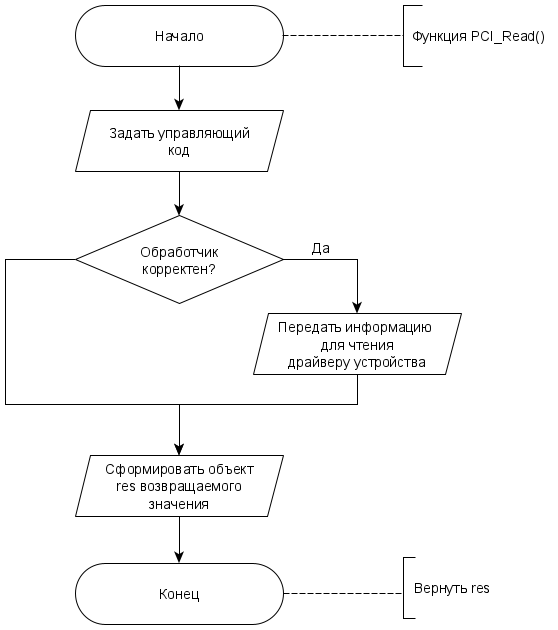
\includegraphics[scale=0.5]{schemes/pci_read.png}}
			\caption{PCI$\_$Read()}
			\label{fig9:image}
		\end{center}
	\end{figure}

	\subsection{Ethernet-КМБО}
	\subsubsection{Функция инициализации (MC$\_$Open)}
	
	Схема изображена на рисунке \ref{fig10:image}.
	
	\begin{figure}[ph!]
		\centering
		\begin{center}
			{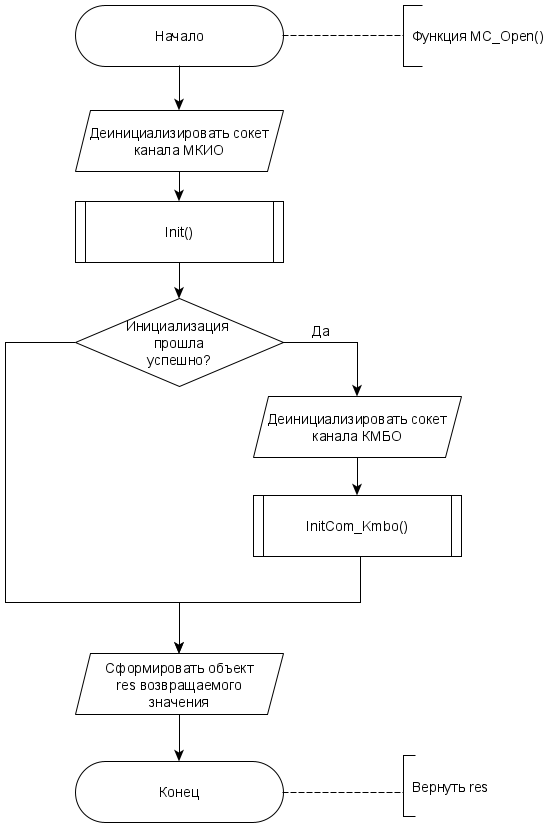
\includegraphics[scale=0.5]{schemes/mc_open.png}}
			\caption{MC$\_$Open()}
			\label{fig10:image}
		\end{center}
	\end{figure}

	\newpage

	\subsubsection{Прекращение работы с MC (MC$\_$Close)}
	
	Схема изображена на рисунке \ref{fig11:image}.
	
	\begin{figure}[ph!]
		\centering
		\begin{center}
			{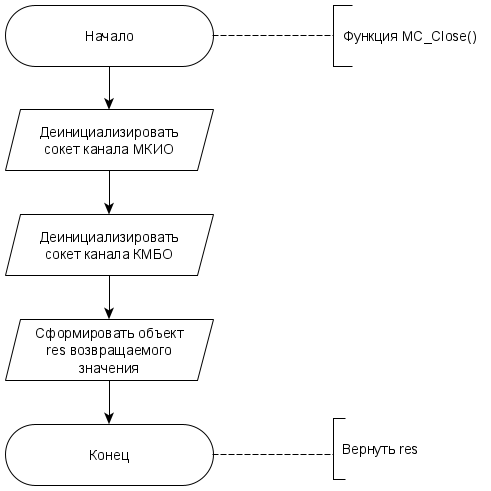
\includegraphics[scale=0.5]{schemes/mc_close.png}}
			\caption{MC$\_$Close()}
			\label{fig11:image}
		\end{center}
	\end{figure}

	\newpage
	\subsubsection{Функция записи данных в устройство MC-КМБО (MC$\_$Write)}
	
	Схема изображена на рисунке \ref{fig12:image}.
	
	\begin{figure}[ph!]
		\centering
		\begin{center}
			{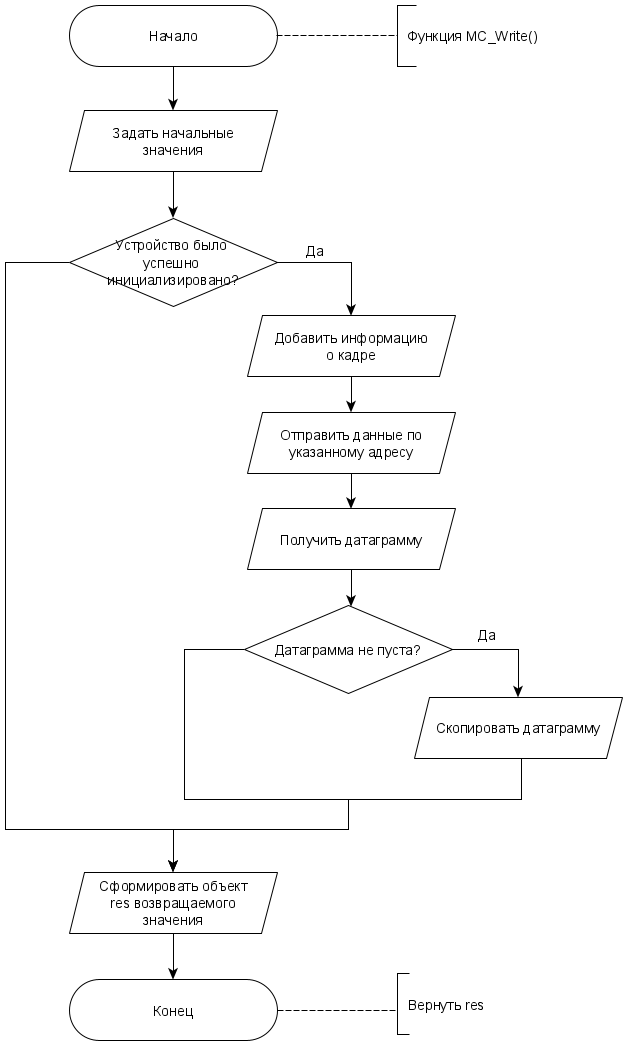
\includegraphics[scale=0.5]{schemes/mc_write.png}}
			\caption{MC$\_$Write()}
			\label{fig12:image}
		\end{center}
	\end{figure}

	\newpage
	\subsubsection{Функция чтения данных из устройства MC-КМБО (MC$\_$Read)}
	
	Схема изображена на рисунке \ref{fig13:image}.
	
	\begin{figure}[ph!]
		\centering
		\begin{center}
			{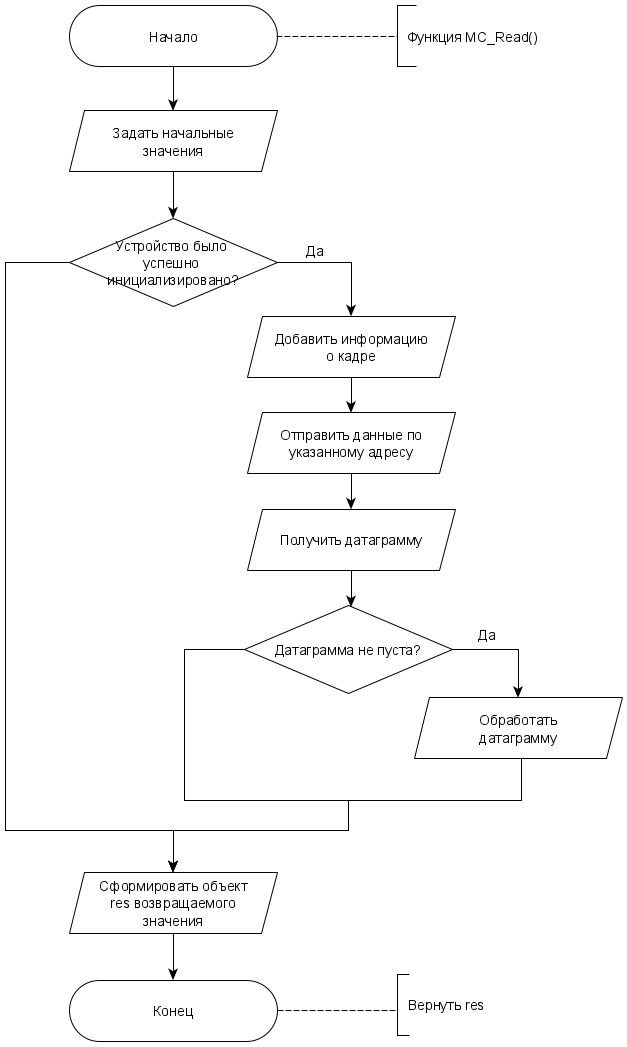
\includegraphics[scale=0.5]{schemes/mc_read.png}}
			\caption{MC$\_$Read()}
			\label{fig13:image}
		\end{center}
	\end{figure}

	\subsubsection{Функция инициализации сокета МКИО (Init)}
	
	Схема изображена на рисунке \ref{fig14:image}.
	
	\begin{figure}[ph!]
		\centering
		\begin{center}
			{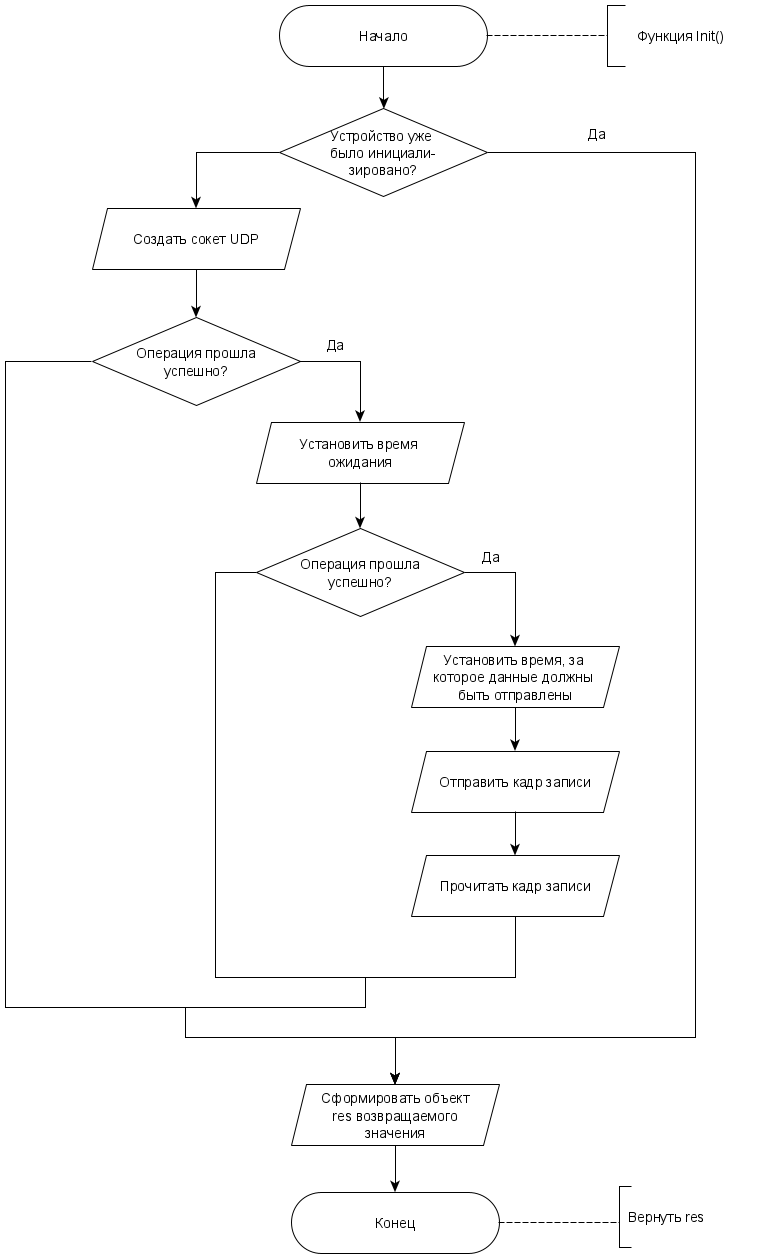
\includegraphics[scale=0.5]{schemes/init.png}}
			\caption{Init()}
			\label{fig14:image}
		\end{center}
	\end{figure}

	\subsubsection{Функция инициализации сокета КМБО (InitCom$\_$Kmbo)}
	
	Схема изображена на рисунке \ref{fig15:image}.
	
	\begin{figure}[ph!]
		\centering
		\begin{center}
			{\includegraphics[scale=0.5]{schemes/InitCom_Kmbо.png}}
			\caption{InitCom$\_$Kmbo()}
			\label{fig15:image}
		\end{center}
	\end{figure}

	\subsection{Вывод}
	В разделе приведены схемы основных функций, входящих в состав библиотеки.

	\newpage
	
%	\setcounter{table}{0}
	\setcounter{figure}{0}
	\newpage
\section{Технологический раздел}
\subsection{Язык программирования}
	При разработке программного продукта был использован язык программирования C$\#$. \cite{c} В качестве среды разработки была использована Visual Studio 2015. \cite{VS2015} Данный выбор обусловлен прежде всего тем, что именно эти инструменты привлекаются для разработки ПО на предприятии. \\
	
	Такой язык программирования был выбран в качестве основного на предприятии по нескольким причинам:
	\begin{enumerate}
		\item [1)] большое количество готовых библиотек и шаблонов;
		\item [2)] исчерпывающая документация;
		\item [3)] низкий порог вхождения;
		\item [4)] поддержка ООП.
	\end{enumerate}

\subsection{Используемые классы}
	На рисунке \ref{fig16:image} представлена UML-диаграмма классов.
	
	\begin{figure}[ph!]
		\centering
		\begin{center}
			{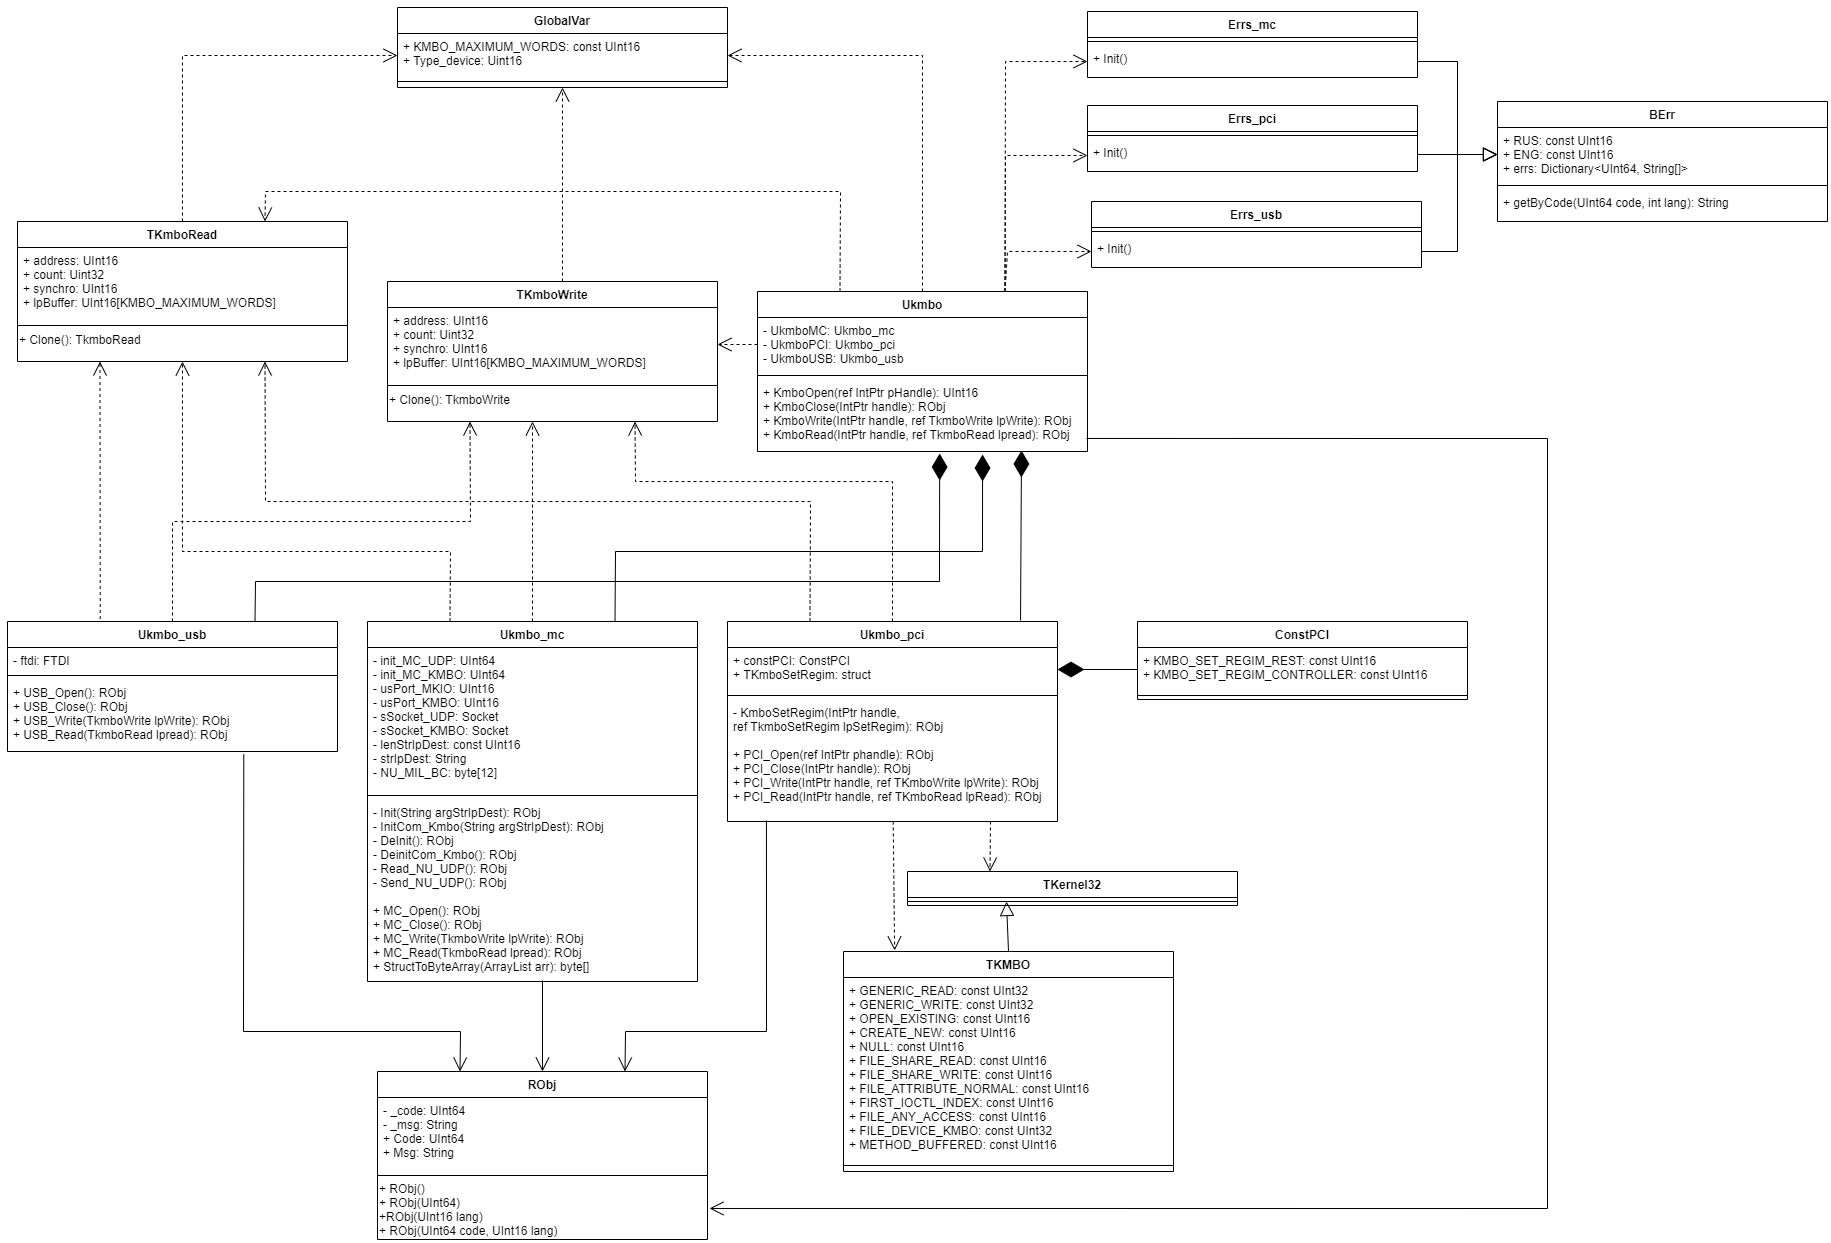
\includegraphics[scale=0.39, angle=90]{schemes/practice.png}}
			\caption{Используемые классы}
			\label{fig16:image}
		\end{center}
	\end{figure}

\newpage

\subsection{Используемые классы}
	\begin{enumerate}
		\item \textbf{Class GlobalVar}
		
		Класс глобальных переменных.
		
		\item \textbf{Class RObj}
		
		Класс возвращаемого значения, хранит код ошибки и соответствующую информацию, заполнение/изменение этого поля происходит одновременно с заданием/изменением поля кода ошибки. 
		
		\item \textbf{Class BErr}
		
		Базовый класс ошибки. Содержит метод getByCode(), который по коду ошибки находит соответствующую информацию о ней, сначала поиск осуществляется по заранее определённому словарю ошибок, в случае неудачи происходит обращение к WinAPI.
		
		\item \textbf{Class Errs$\_$mc}
		
		Класс ошибок, определённых для MC.
		
		\item \textbf{Class Errs$\_$usb}
		
		Класс ошибок, определённых для USB.
		
		\item \textbf{Class Errs$\_$pci}
		
		Класс ошибок, определённых для PCI.
		
		\item \textbf{Class TKMBO}
		
		Содержит необходимые для работы константы.
		
		\item \textbf{Class TKmboRead}
		
		Класс данных для чтения. \\
		Содержит поля адреса, количества записываемых слов, флаг, который определяет будет ли выводиться сигнал на осциллограф или нет и массив записанных слов.
		
		\item \textbf{Class TKmboWrite}
		
		Класс данных для записи. \\
		Содержит поля адреса, количества записываемых слов, флаг, который определяет будет ли выводиться сигнал на осциллограф или нет и массив записанных слов.
		
		\item \textbf{Class Ukmbo}
		
		Содержит основные методы взаимодействия с КМБО, такие как Open, Close, Read, Write.
		
		\item \textbf{Class Ukmbo$\_$mc}
		
		Содержит методы для взаимодействия с МС.
		
		\item \textbf{Class Ukmbo$\_$usb}
		
		Содержит методы для взаимодействия с USB.
		
		\item \textbf{Class ConstPCI}
		
		Класс констант, необходимых для взаимодействия с шиной PCI.
		
		\item \textbf{Class Ukmbo$\_$pci}
		
		Содержит методы для взаимодействия с PCI.
	\end{enumerate}

		Программная реализация классов представлена в приложениях А-Д.
		
	\subsection{Вывод}
	В этом разделе обосновывается выбор языка программирования и среды разработки, рассмотрена UML-диаграмма основных классов.



	\newpage
	
	\section*{Заключение}
\addcontentsline{toc}{section}{Заключение}
Во время прохождения практики была достигнута поставленная цель, а именно, была разработана и отлажена библиотека алгоритмов взаимодействия персонального компьютера и контрольной измерительной аппаратурой радиолокационной головкой самонаведения. \\

В процессе выполнения были решены все задачи: изучены алгоритмы взаимодействия ПК и КИА РГС, протокол канала межблочного обмена, проработаны особенности взаимодействия с PCI, USB и Ethernet. В результате была разработана соответствующая библиотека алгоритмов, которая впоследствии была успешно отлажена.

	\newpage
	
	\newpage
	\begin{thebibliography}{9} 
		\addcontentsline{toc}{section}{Литература}
		
		\bibitem{book1} Военный энциклопедический словарь / Пред. Гл. ред. комиссии: С.Ф. Ахромеев. – 2-е изд. – М.: Воениздат, 1986. – 863 с. – 150 000 экз.
		
		\bibitem{book2} Куркоткин В.И., Стерлингов В.Л. Самонаведение ракет. – М.: Воениздат, 1963. – 92 с. – (Ракетная техника). – 20 000 экз. 
		
		\bibitem{kmbo} Контроллер канала межблочного обмена [Электронный ресурс]. – Режим доступа: https://findpatent.ru/patent/234/2345407.html    (дата обращения 01.07.2021).
		
		\bibitem{FT2232H} Основные особенности микросхемы FT2232H [Электронный ресурс]. – Режим доступа: http://microsin.net/adminstuff/hardware/ft2232h-dual-uart-fifo-usb-converter.html  (дата обращения 05.07.2021)
		
		\bibitem{ftdi} FTDI [Электронный ресурс]. – Режим доступа: https://ftdichip.com/  (дата обращения 05.07.2021)
		
		\bibitem{mc} Микросхема mc [Электронный ресурс]. – Режим доступа: http://hardelectronics.ru/mc34063.html (дата обращения 07.07.2021)
		
		\bibitem{c} Документация по С\# [Электронный ресурс]. – Режим доступа: https://docs.microsoft.com/ru-ru/dotnet/csharp/  (дата обращения 02.07.2021)
		
		\bibitem{VS2015} Документация по Visual Studio 2015 [Электронный ресурс]. – Режим доступа: https://docs.microsoft.com/ru-ru/visualstudio/vs-2015-archive?view=vs-2019   (дата обращения 07.07.2021)
		
		
		
		
	\end{thebibliography}
	\newpage
	
	\section*{\hfill Приложение А \hfill}
\addcontentsline{toc}{section}{Приложение А}
Приведены листинги основных классов.

\begin{lstlisting}[label=kmbo,caption=Основные функции КМБО]
namespace Kmbo
{
	public class GlobalVar
	{
		public const int KMBO_MAXIMUM_WORDS = 64;      
		public static int Type_Device = -1;
	}
	
	public class TKMBO : TKernel32
	{
		public const UInt32 GENERIC_READ = 0x80000000;
		public const UInt32 GENERIC_WRITE = 0x80000000;
		public const UInt16 OPEN_EXISTING = 3;
		const UInt16 CREATE_NEW = 1;
		public const UInt16 NULL = 0;
		public const UInt16 FILE_SHARE_READ = 0;
		public const UInt16 FILE_SHARE_WRITE = 0;
		public const UInt16 FILE_ATTRIBUTE_NORMAL = 0;
		public const UInt16 FIRST_IOCTL_INDEX = 0x0800;
		public const UInt16 FILE_ANY_ACCESS = 0x0000;
		public const UInt32 FILE_DEVICE_KMBO = 0x00008000;
		public const UInt16 METHOD_BUFFERED = 0;
		const UInt16 METHOD_IN_DIRECT = 1;
		const UInt16 METHOD_OUT_DIRECT = 2;
		const UInt16 METHOD_NEITHER = 3;
		const UInt16 REGIM_REST = 0;                                         
		const UInt16 REGIM_CONTROLLER = 0x1;                              
	}
	
	public class TKmboRead
	{
		public UInt16 address;                         
		public UInt32 count;                            
		public UInt16 synchro;                          
		public UInt16[] lpBuffer = new UInt16[GlobalVar.KMBO_MAXIMUM_WORDS];
		
		public object Clone()
		{
			UInt16[] temp = new UInt16[this.lpBuffer.Length];
			Array.Copy(this.lpBuffer, temp, this.lpBuffer.Length);
			
			return new TKmboRead
			{
				address = this.address,
				count = this.count,
				synchro = this.synchro,
				lpBuffer = temp
			};
		}
	}
	
	public class TKmboWrite                             
	{
		public UInt16 address;                          
		public UInt32 count;                            
		public UInt16 synchro;                          
		public UInt16[] lpBuffer = new UInt16[GlobalVar.KMBO_MAXIMUM_WORDS];    
		
		public object Clone()
		{
			UInt16[] temp = new UInt16[this.lpBuffer.Length];
			Array.Copy(this.lpBuffer, temp, this.lpBuffer.Length);
			
			return new TKmboWrite
			{
				address = this.address,
				count = this.count,
				synchro = this.synchro,
				lpBuffer = temp
			};
		}
	}
	
	public class Ukmbo
	{
		Ukmbo_mc UkmboMC = new Ukmbo_mc();
		Ukmbo_usb UkmboUSB = new Ukmbo_usb();
		Ukmbo_pci UkmboPCI = new Ukmbo_pci();
		public int KmboOpen(ref IntPtr pHandle)
		{
			Errs_mc.Init();
			
			if (UkmboMC.MC_Open().Code == 0)
			{
				pHandle = (IntPtr)null;
				GlobalVar.Type_Device = 2;
			}
			else
			{
				ErrsUSB.Init();
				
				if (UkmboUSB.USB_Open().Code == 0)
				GlobalVar.Type_Device = 1;
				else
				{
					ErrsPCI.Init();
					
					if (UkmboPCI.PCI_Open(ref pHandle).Code == 0)
					GlobalVar.Type_Device = 0;
					else
					GlobalVar.Type_Device = -1;
				}
			}
			
			return GlobalVar.Type_Device;
		}
		
		public RObj KmboClose(IntPtr handle)
		{
			RObj res = new RObj();
			
			switch (GlobalVar.Type_Device)
			{
				case 0:
				res.Code = UkmboPCI.PCI_Close(handle).Code;
				break;
				case 1:
				res.Code = UkmboUSB.USB_Close().Code;
				break;
				case 2:
				res.Code = UkmboMC.MC_Close().Code;
				break;
			}
			
			return res;
		}
		
		public RObj KmboWrite(IntPtr handle, ref TKmboWrite lpWrite)
		{
			
			RObj res = new RObj();
			
			switch (GlobalVar.Type_Device)
			{
				case 0:
				res.Code = UkmboPCI.PCI_Write(handle, ref lpWrite).Code;
				break;
				case 1:
				res.Code = UkmboUSB.USB_Write(lpWrite).Code;
				break;
				case 2:
				res.Code = UkmboMC.MC_Write(lpWrite).Code;
				break;
			}
			return res;
		}
		
		public RObj KmboRead(IntPtr handle, ref TKmboRead lpRead)
		{
			RObj res = new RObj();
			
			switch (GlobalVar.Type_Device)
			{
				case 0:
				res.Code = UkmboPCI.PCI_Read(handle, ref lpRead).Code;
				break;
				case 1:
				res.Code = UkmboUSB.USB_Read(ref lpRead).Code;
				break;
				case 2:
				res.Code = UkmboMC.MC_Read(lpRead).Code;
				break;
			}
			return res;
		}
	}
}
\end{lstlisting}
	
	\newpage
	
	\section*{\hfill Приложение Б \hfill}
\addcontentsline{toc}{section}{Приложение Б}
Приведены листинги методов, связанных с MC.

\begin{lstlisting}[label=mc,caption=Основные функции взаимодействия с MC]
namespace Kmbo
{
	public class Ukmbo_mc
	{
		static UInt64 init_MC_UDP = 0xC0000007L;         
		static UInt64 init_MC_Kmbo = 0xC0000007L;        
		
		static int usPort_MKIO = 0x4001;                 
		static int usPort_KMBO = 0x4002;                 
		
		static Socket sSocket_UDP;
		static Socket sSocket_KMBO;
		
		const int lenStrIpDest = 16;
		static string strIpDest;
		
		static byte[] NU_MIL_BC = new byte[12] { 0xCD, 0xAB, 0x01, 0x00, 0x01, 0x00,
			0x01, 0x00, 0x15, 0x00, 0xBA, 0xDC };
		public static long time_on_wr;
		public static long time_on_rd;
		long time_max_wr = 0;
		long time_max_rd = 0;
		
		public RObj MC_Open()
		{
			RObj res = new RObj();
			
			Deinit();
			if (Init("192.168.1.71").Code == 0) 
			{
				DeinitCom_Kmbo();
				res.Code = (ulong)InitCom_Kmbo("192.168.1.71").Code;
			}
			else
			{
				res.Code = 0xC0000006L;
			}
			
			return res;
		}
		public RObj MC_Close()
		{
			RObj res = new RObj();
			
			res.Code = Deinit().Code;
			res.Code += DeinitCom_Kmbo().Code;
			
			return res;
		}
		public RObj MC_Read(TKmboRead argData)
		{
			long li_Freq;
			Stopwatch stopwatch;
			long li_TimeNow;
			
			byte[] bufferReceive = new byte[1460];
			UInt16[] bf_Receive = new UInt16[730];
			
			int result = 0;
			UInt16 Number_Frame_KMBO = 0;
			
			TKmboRead kr = (TKmboRead)argData.Clone();
			
			EndPoint ipSender;
			IPEndPoint ipDest;
			
			try
			{
				ipSender = new IPEndPoint(IPAddress.Any, 0);
			}
			catch (SocketException ex)
			{
				Console.WriteLine("ERROR: " + ex.ToString() + "\n" + ex.Message);
				return new RObj(0xC0000005L);
			}
			
			RObj res = new RObj(0xC0000007L);
			
			if (init_MC_Kmbo != 0) 
			{
				return res;
			}
			
			ArrayList al = new ArrayList();
			
			al.Add((UInt16)0xabcd);
			al.Add((UInt16)0x0000);
			al.Add((UInt16)0x0001);
			
			al.Add((UInt16)(kr.count & 0x00ff));
			al.Add((UInt16)(((kr.address << 8) & 0xff00) | 0x0080));
			
			Number_Frame_KMBO++;
			
			al[2] = (UInt16)Number_Frame_KMBO;
			al.Add((UInt16)0xdcba);
			
			try
			{
				ipDest = new IPEndPoint(IPAddress.Parse(strIpDest), usPort_KMBO);
			}
			catch (SocketException ex)
			{
				Console.WriteLine("ERROR: " + ex.ToString() + "\n" + ex.Message);
				return new RObj(0xC0000005L);
			}
			
			sSocket_KMBO.SendTo(StructToByteArray(al), ipDest);
			
			result = sSocket_KMBO.ReceiveFrom(bufferReceive, ref ipSender);
			
			if (result > 0)
			{
				Buffer.BlockCopy(bufferReceive, 0, bf_Receive, 0, bufferReceive.Length);
				
				if (bf_Receive[0] == 0xabcd)
				{
					for (int i = 4; i < bf_Receive.Length / 2; i++)
					{
						if ((bf_Receive[i] & 0xff00) == ((kr.address << 8) & 0xff00))
						{
							Buffer.BlockCopy(bf_Receive, i + 1, kr.lpBuffer, 0, (int)kr.count);
							
							kr = argData;
							res.Code = 0;
							break;
						}
						if (bf_Receive[i] == 0xdcba)
						{
							break;
						}
					}
				}
			}
			
			return res;
		}
		public RObj MC_Write(TKmboWrite argData)
		{
			long li_Freq;
			Stopwatch stopwatch;
			long li_TimeNow;
			
			RObj res = new RObj(0xC0000007L);
			
			byte[] bufferReceive = new byte[1460];
			UInt16[] bf_Receive = new UInt16[730];
			
			int result;
			UInt16 Number_Frame_KMBO = 0;
			
			TKmboWrite wr = (TKmboWrite)argData.Clone();
			
			EndPoint ipSender;
			
			try
			{
				ipSender = new IPEndPoint(IPAddress.Any, 0);
			}
			catch (SocketException ex)
			{
				Console.WriteLine("ERROR: " + ex.ToString() + "\n" + ex.Message);
				return new RObj(0xC0000005L);
			}
			
			if (init_MC_Kmbo != 0)
			{
				return res;
			}
			
			ArrayList al = new ArrayList();
			
			al.Add((UInt16)0xabcd);
			al.Add((UInt16)0x0000);
			al.Add((UInt16)0x0001);
			
			al.Add((UInt16)(wr.count & 0x00ff));
			al.Add((UInt16)((wr.address << 8) & 0xff00));
			
			for (int i = 0; i < wr.count; i++) al.Add(wr.lpBuffer[i]);
			Number_Frame_KMBO++;
			
			al[2] = (UInt16)Number_Frame_KMBO;
			al.Add((UInt16)0xdcba);
			
			IPEndPoint ipDest;
			
			try
			{
				ipDest = new IPEndPoint(IPAddress.Parse(strIpDest), usPort_KMBO);
			}
			catch (SocketException ex)
			{
				Console.WriteLine("ERROR: " + ex.ToString() + "\n" + ex.Message);
				return new RObj(0xC0000005L);
			}
			
			sSocket_KMBO.SendTo(StructToByteArray(al), ipDest);
			
			result = sSocket_KMBO.ReceiveFrom(bufferReceive, ref ipSender);
			
			if (result > 0)
			{
				Buffer.BlockCopy(bufferReceive, 0, bf_Receive, 0, bufferReceive.Length);
				if (bf_Receive[0] == 0xabcd) res.Code = 0;
			}
			
			return res;
		}
		
		private RObj Init(string argStrIpDest)
		{
			if (init_MC_UDP == 0) return new RObj(0);
			
			strIpDest = argStrIpDest;
			
			try
			{
				sSocket_UDP = new Socket(AddressFamily.InterNetwork, SocketType.Dgram, ProtocolType.Udp);
			}
			catch (SocketException ex)
			{
				Console.WriteLine("ERROR: " + ex.ToString() + "\n" + ex.Message);
				return new RObj(0xC0000001L);
			}
			
			try
			{
				sSocket_UDP.ReceiveTimeout = 50; 
			}
			catch (SocketException ex)
			{
				Console.WriteLine("ERROR: " + ex.ToString() + "\n" + ex.Message);
				return new RObj(0xC0000003L);
			}
			
			try
			{
				sSocket_UDP.SendTimeout = 50;
			}
			catch (SocketException ex)
			{
				Console.WriteLine("ERROR: " + ex.ToString() + "\n" + ex.Message);
				return new RObj(0xC0000004L);
			}
			
			Send_NU_UDP();
			init_MC_UDP = Read_NU_UDP().Code;
			
			return new RObj(init_MC_UDP);
		}
		
		private RObj Send_NU_UDP()
		{
			IPEndPoint ipDest;
			
			try
			{
				ipDest = new IPEndPoint(IPAddress.Parse(strIpDest), usPort_MKIO);
			}
			catch (SocketException ex)
			{
				Console.WriteLine("ERROR: " + ex.ToString() + "\n" + ex.Message);
				return new RObj(0xC0000005L);
			}
			
			sSocket_UDP.SendTo(NU_MIL_BC, ipDest);
			
			return new RObj(0);
		}
		private RObj Read_NU_UDP()
		{
			int result;
			EndPoint remoteIP;
			
			try
			{
				remoteIP = new IPEndPoint(IPAddress.Any, 0);
			}
			catch (SocketException ex)
			{
				Console.WriteLine("ERROR: " + ex.ToString() + "\n" + ex.Message);
				return new RObj(0xC0000005L);
			}
			
			byte[] bufferReceive = new byte[1460];
			StringBuilder str = new StringBuilder();
			
			result = sSocket_UDP.ReceiveFrom(bufferReceive, ref remoteIP);
			
			if (result > 0)
			{
				str.Append(Encoding.Unicode.GetString(bufferReceive, 0, result));
				return new RObj(0);
			}
			else return new RObj(0xC0000008L);
		}
		
		private RObj Deinit()
		{
			if (init_MC_UDP != 0) return new RObj(0xC0000007L);
			
			sSocket_UDP.Close();
			init_MC_UDP = 0xC0000007L;
			
			return new RObj(init_MC_UDP);
		}
		
		private RObj InitCom_Kmbo(string argStrIpDest)
		{
			RObj result = new RObj();
			EndPoint ipAddr;
			
			if (init_MC_Kmbo == 0) return result;
			
			strIpDest = argStrIpDest;
			
			try
			{
				sSocket_KMBO = new Socket(AddressFamily.InterNetwork, SocketType.Dgram, ProtocolType.Udp);
			}
			catch (SocketException ex)
			{
				Console.WriteLine("ERROR: " + ex.ToString() + "\n" + ex.Message);
				return new RObj(0xC0000001L);
			}
			
			try
			{
				ipAddr = new IPEndPoint(IPAddress.Any, 0x5003);
			}
			catch (SocketException ex)
			{
				Console.WriteLine("ERROR: " + ex.ToString() + "\n" + ex.Message);
				return new RObj(0xC0000005L);
			}
			
			try
			{
				sSocket_KMBO.Bind(ipAddr);
			}
			catch (SocketException ex)
			{
				Console.WriteLine("ERROR: " + ex.ToString() + "\n" + ex.Message);
				return new RObj(0xC0000002L);
			}
			
			init_MC_Kmbo = 0;
			
			return result;
		}
		
		private RObj DeinitCom_Kmbo()
		{
			if (init_MC_Kmbo != 0) return new RObj(0xC0000007L);
			
			sSocket_KMBO.Close();
			
			init_MC_Kmbo = 0xC0000007L;
			
			return new RObj(init_MC_Kmbo);
		}
		
		static public byte[] StructToByteArray(ArrayList arr)
		{
			object[] obj = (arr.ToArray());
			
			int sizeInBytes;
			
			byte[] outByte = new byte[0];
			
			for (int i = 0; i < obj.Count(); i++)
			{
				sizeInBytes = Marshal.SizeOf(obj[i]);
				
				byte[] outArray = new byte[sizeInBytes];
				
				IntPtr ptr = Marshal.AllocHGlobal(sizeInBytes);
				
				Marshal.StructureToPtr(obj[i], ptr, true);
				Marshal.Copy(ptr, outArray, 0, sizeInBytes);
				Marshal.FreeHGlobal(ptr);
				outByte = outByte.Concat(outArray).ToArray();
			}
			return outByte;
		}
	}
}
\end{lstlisting}
	\newpage
	
	\section*{\hfill Приложение В \hfill}
\addcontentsline{toc}{section}{Приложение В}
Приведены листинги методов, связанных с PCI.

\begin{lstlisting}[label=pci,caption=Основные функции взаимодействия с PCI]
namespace Kmbo
{
	public class Ukmbo_pci
	{
		public class ConstPCI
		{
			public const int KMBO_SET_REGIM_REST = 0;		    
			public const int KMBO_SET_REGIM_CONTROLLER = 0x1;	
		}
		public struct TKmboSetRegim
		{
			public ulong regim;                                
		}
		public RObj PCI_Open(ref IntPtr pHandle)
		{
			TKmboSetRegim SetRegim;
			pHandle = TKernel32.CreateFile("\\\\.\\kmbo",
			TKMBO.GENERIC_READ | TKMBO.GENERIC_WRITE,
			TKMBO.FILE_SHARE_READ | TKMBO.FILE_SHARE_WRITE,
			TKMBO.NULL,
			TKMBO.OPEN_EXISTING,
			TKMBO.FILE_ATTRIBUTE_NORMAL,
			TKMBO.NULL);
			if (pHandle == (IntPtr)(-1))
			return new RObj(TKernel32.GetLastError());
			
			SetRegim.regim = ConstPCI.KMBO_SET_REGIM_CONTROLLER;
			return KmboSetRegim(pHandle, ref SetRegim);
		}
		public RObj PCI_Close(IntPtr handle)
		{
			RObj res = new RObj();
			
			if (handle != (IntPtr)(-1))                         
			{
				if (TKernel32.CloseHandle(handle) == false)
				res.Code = TKernel32.GetLastError();
				return res;
			}
			return res;
		}
		unsafe public RObj PCI_Write(IntPtr handle, ref TKmboWrite lpWrite)
		{
			UInt32 ret = 0;
			RObj res = new RObj();
			
			UInt32 lu_SetRegime = (UInt32)((TKMBO.FILE_DEVICE_KMBO << 16) | 
			(TKMBO.FILE_ANY_ACCESS << 14) |
			((TKMBO.FIRST_IOCTL_INDEX + 1) << 2) | 
			(TKMBO.METHOD_BUFFERED)); //+1 attention
			
			if (handle != (IntPtr)(-1))
			{
				fixed (UInt16* Arr = &lpWrite.address)
				{
					if (!TKernel32.DeviceIoControl(handle,
					lu_SetRegime,
					(UInt16*)Arr,
					(UInt32)Marshal.SizeOf(typeof(TKmboWrite)),
					null,
					0,
					&ret,
					TKMBO.NULL))
					res.Code = TKernel32.GetLastError();
				}
			}
			return res;
		}
		unsafe public RObj PCI_Read(IntPtr handle, ref TKmboRead lpRead)
		{
			UInt32 ret;
			RObj res = new RObj();
			
			UInt32 lu_SetRegime = (UInt32)((TKMBO.FILE_DEVICE_KMBO << 16) | 
			(TKMBO.FILE_ANY_ACCESS << 14) |
			((TKMBO.FIRST_IOCTL_INDEX) << 2) | 
			(TKMBO.METHOD_BUFFERED)); 
			if (handle != (IntPtr)(-1))
			{
				fixed (UInt16* Arr = &lpRead.address)
				{
					if (!TKernel32.DeviceIoControl(handle,
					lu_SetRegime,
					(UInt16*)Arr,
					(UInt32)Marshal.SizeOf(typeof(TKmboRead)),
					(UInt16*)Arr,
					(UInt32)Marshal.SizeOf(typeof(TKmboRead)),
					&ret,
					TKMBO.NULL))
					res.Code = TKernel32.GetLastError();
				}
			}
			return res;
		}
		
		unsafe RObj KmboSetRegim(IntPtr handle, ref TKmboSetRegim lpSetRegim)
		{
			UInt32 ret;
			RObj res = new RObj();
			
			if (handle != (IntPtr)(-1))
			{
				UInt32 lu_SetRegime = (UInt32)((TKMBO.FILE_DEVICE_KMBO << 16) | 
				(TKMBO.FILE_ANY_ACCESS << 14) |
				((TKMBO.FIRST_IOCTL_INDEX + 5) << 2) | 
				(TKMBO.METHOD_BUFFERED));
				
				fixed (TKmboSetRegim* Arr = &lpSetRegim)
				{
					if (!TKernel32.DeviceIoControl(handle,
					lu_SetRegime,
					(UInt16*)Arr,
					(UInt32)Marshal.SizeOf(typeof(TKmboSetRegim)),
					null,
					0,
					&ret,
					TKMBO.NULL))
					res.Code = TKernel32.GetLastError();
				}
			}
			return res;
		}
	}
}
\end{lstlisting}
	\newpage
	
	\section*{\hfill Приложение Г \hfill}
\addcontentsline{toc}{section}{Приложение Г}
Приведены листинги методов, связанных с USB.

\begin{lstlisting}[label=usb,caption=Основные функции взаимодействия с USB]
namespace Kmbo
{
	class Ukmbo_usb
	{
		FTDI ftdi = new FTDI();
		
		public RObj USB_Open()
		{
			FTDI.FT_STATUS ftStatus;                                    
			
			ftStatus = ftdi.OpenByDescription("USB <-> Serial Cable A");
			
			if (ftStatus == FTDI.FT_STATUS.FT_OK)                      
			{
				ftStatus = ftdi.ResetDevice();                          
				if (ftStatus != FTDI.FT_STATUS.FT_OK) return new RObj((ulong)ftStatus); 
				
				ftStatus = ftdi.SetBitMode(0xff, 0x00);                 
				if (ftStatus != FTDI.FT_STATUS.FT_OK) return new RObj((ulong)ftStatus);   
				
				ftStatus = ftdi.SetTimeouts(1, 1);
				if (ftStatus != FTDI.FT_STATUS.FT_OK) return new RObj((ulong)ftStatus);
				
				return new RObj(0);
			}
			else return new RObj(2);
		}
		
		public RObj USB_Close()
		{
			return new RObj((ulong)ftdi.Close());
		}
		
		public RObj USB_Write(TKmboWrite lpWrite)
		{
			UInt64 res = 0;
			Int16 Reg = 0;
			FTDI.FT_STATUS ftStatus;
			
			UInt16 Adr;
			UInt16 N;
			UInt16[] m = new ushort[62];
			bool s;
			
			Adr = lpWrite.address;
			N = (UInt16)lpWrite.count;
			
			Buffer.BlockCopy(lpWrite.lpBuffer, 0, m, 1, (int)(lpWrite.count * sizeof(UInt16)));
			
			if (lpWrite.synchro == 1) s = true;
			else s = false;
			
			UInt32 RxBytes;                             
			byte[] TxBuffer = new byte[256];            
			byte[] RxBuffer = new byte[2];              
			UInt32 dwBytesToWrite = 0;                  
			UInt32 dwBytesWritten = 0;                  
			UInt32 dwBytesReceived = 0;                
			
			if (N > 62) N = 62;
			m[0] = (UInt16)((Adr << 8) + (N << 1));
			
			UInt16 n = 0;
			UInt16 a;
			
			for (int i = 1; i <= 15; i++)               
			{
				a = (UInt16)(m[0] >> i);
				if ((a & 0x0001) == 0x0001) n++;
			}
			if (n % 2 == 0) m[0]++;
			
			dwBytesToWrite = (UInt32)(N + 1) * 2 + 1;   
			Reg |= 1;                                   
			
			if (s == false) Reg &= ~2;
			else Reg |= 2;
			
			TxBuffer[0] = (byte)Reg;
			for (int i = 1; i <= ((N + 1) * 2); i++)
			if (i % 2 == 0)
			TxBuffer[i] = (byte)(m[(i >> 1) - 1] & 0x00FF);
			else
			TxBuffer[i] = (byte)(m[i >> 1] >> 8);
			
			ftStatus = ftdi.Write(TxBuffer, dwBytesToWrite, ref dwBytesWritten);
			if (ftStatus != FTDI.FT_STATUS.FT_OK) return new RObj((ulong)ftStatus); 
			
			RxBytes = 1;
			ftStatus = ftdi.Read(RxBuffer, RxBytes, ref dwBytesReceived);
			if (ftStatus != FTDI.FT_STATUS.FT_OK) return new RObj((ulong)ftStatus);
			
			if (RxBytes != dwBytesReceived) res = 19;   
			if ((RxBuffer[0] & 0xF9) != 0x20) res = 20; 
			if ((RxBuffer[0] & 0x04) == 0x04) res = 21; 
			if ((RxBuffer[0] & 0x02) == 0x02) res = 22; 
			
			return new RObj(res);
		}
		
		public RObj USB_Read(ref TKmboRead lpRead)
		{
			UInt64 res = 0;
			Int16 Reg = 0;
			FTDI.FT_STATUS ftStatus;
			
			UInt16 Adr;
			UInt16 N;
			UInt16[] m = new UInt16[62];
			bool s;
			
			Adr = lpRead.address;
			N = (UInt16)lpRead.count;
			if (lpRead.synchro == 1) s = true;
			else s = false;
			
			UInt32 RxBytes;                             
			byte[] TxBuffer = new byte[3];              
			byte[] RxBuffer = new byte[129];           
			UInt32 dwBytesToWrite = 0;                 
			UInt32 dwBytesWritten = 0;                  
			UInt32 dwBytesReceived = 0;                 
			
			if (N > 63) N = 0;
			m[0] = (UInt16)((Adr << 8) + (N << 1) + 0x0080);
			
			UInt16 n = 0;
			UInt16 a;
			
			for (int i = 1; i <= 15; i++)               
			{
				a = (UInt16)(m[0] >> i);
				if ((a & 0x0001) == 0x0001) n++;
			}
			if (n % 2 == 0) m[0]++;
			
			if (N == 0) N = 64;
			dwBytesToWrite = 3;                         
			Reg |= 1;                                   
			
			if (s == false) Reg &= ~2;
			else Reg |= 2;
			TxBuffer[0] = (byte)Reg;
			TxBuffer[1] = (byte)(m[0] >> 8);
			TxBuffer[2] = (byte)(m[0] & 0x00FF);
			
			ftStatus = ftdi.Write(TxBuffer, dwBytesToWrite, ref dwBytesWritten);
			if (ftStatus != FTDI.FT_STATUS.FT_OK) return new RObj((ulong)ftStatus);
			
			RxBytes = (UInt32)(2 * N + 1);
			ftStatus = ftdi.Read(RxBuffer, RxBytes, ref dwBytesReceived);
			if (ftStatus != FTDI.FT_STATUS.FT_OK) return new RObj((ulong)ftStatus);
			if (RxBytes != dwBytesReceived) res = 19;   
			
			for (int i = 1; i <= N; i++)                
			m[i] = (UInt16)((RxBuffer[2 * i - 2] << 8) +(RxBuffer[2 * i - 1] & 0x00FF));
			
			Buffer.BlockCopy(m, 1, lpRead.lpBuffer, 0, (int)(lpRead.count * sizeof(UInt16)));
			
			if ((RxBuffer[2 * N] & 0xF9) != 0x20) res = 20; 
			if ((RxBuffer[2 * N] & 0x04) == 0x04) res = 21; 
			if ((RxBuffer[2 * N] & 0x02) == 0x02) res = 22; 
			
			return new RObj(res);
		}
	}
}
\end{lstlisting}
	\newpage
	
	\section*{\hfill Приложение Д \hfill}
\addcontentsline{toc}{section}{Приложение Д}
Приведены листинги классов, описывающих ошибки.

\begin{lstlisting}[label=err,caption=Ошибки]
namespace Errs
{
	public class BErr
	{
		public const int RUS = 0;
		public const int ENG = 1;
		
		public static Dictionary<UInt64, String[]> errs;
		
		public static String getByCode(UInt64 code, int lang)
		{
			if (errs.ContainsKey(code))
				return "Code = " + code.ToString() + ". " + errs[code][0];
			else
			{
				IntPtr lpMsgBuf = IntPtr.Zero;
				
				if (TKernel32.FormatMessage(TKernel32.FormatMessageFlags.FORMAT_MESSAGE_ALLOCATE_BUFFER |
				TKernel32.FormatMessageFlags.FORMAT_MESSAGE_FROM_SYSTEM |
				TKernel32.FormatMessageFlags.FORMAT_MESSAGE_IGNORE_INSERTS,
				IntPtr.Zero,
				(uint)code,
				0,
				ref lpMsgBuf,
				0,
				IntPtr.Zero) == 0)
					return "Code = " + code.ToString() + ". Not defined mistake";
				
				return "Code = " + code.ToString() + ". " + Marshal.PtrToStringAnsi(lpMsgBuf);
			}
		}
		
		public static void Add(UInt64 code, String msgEng, String msgRus)
		{
			errs.Add(code, new String[2] { msgEng, msgRus });
		}
	}
	
	public class RObj
	{
		private UInt64 _code = 0;
		private String _msg;
		
		public UInt64 Code
		{
			get
			{
				return _code;
			}
			
			set
			{
				_code = value;
				_msg = BErr.getByCode(_code, BErr.ENG);
			}
		}
		
		public String Msg
		{
			get
			{
				return _msg;
			}
		}
		
		public RObj()
		{
			_msg = BErr.getByCode(_code, BErr.ENG);
		}
		
		public RObj(UInt64 code)
		{
			this._code = code;
			_msg = BErr.getByCode(code, BErr.ENG);
		}
		
		public RObj(int lang)
		{
			_msg = BErr.getByCode(_code, lang);
		}
		
		public RObj(UInt64 code, int lang)
		{
			this._code = code;
			_msg = BErr.getByCode(code, lang);
		}
	}

	public class Errs_mc : BErr
	{
		static public void Init()
		{
			if (errs != null)
			errs.Clear();
			
			errs = new Dictionary<UInt64, String[]>()
			{
				[0] = new String[2]{ "OK"},
				
				[0xC0000001L] = new String[2] { "Creation of socket for transfering data was FAILED"},
				
				[0xC0000002L] = new String[2] { "Binding a socket was FAILED, error in calling function 'bind'"},
				
				[0xC0000003L] = new String[2] { "Error in setting timeout for receiving the data from clients to socket"},
				
				[0xC0000004L] = new String[2] { "Error in setting timeout for sending the data to clients from socket"},
				
				[0xC0000005L] = new String[2] { "Error in creation of connection point"},
				
				[0xC0000006L] = new String[2] { "Connection with mc was FAILED"},
				
				[0xC0000007L] = new String[2] { "Error in initialization of module mc"},
				
				[0xC0000008L] = new String[2] { "There is no available data"},
				
			};
		}
	}

    public class ErrsPCI : BErr
	{                        
		static public void Init()
		{
			if (errs != null)
			errs.Clear();
			
			errs = new Dictionary<UInt64, String[]>()
			{
				[0] = new String[2]{ "OK"},
				
				[0xE0000001L] = new String[2]{ "The zero-length buffer was passed to the driver for receiving/transmitting"},
				
				[0xE0000002L] = new String[2]{ "The buffer with too large length was passed to the driver for receiving/transmitting"},
				
				[0xE0000003L] = new String[2]{ "The buffer with incorrect length was passed to the driver for executing command"},
				
				[0xE0000004L] = new String[2]{ "The incorrect data was passed to the driver for executing command"},
				
				[0xE0000005L] = new String[2]{ "The attribute 'Counter work' was set after the exchange"},
				
				[0xE0000006L] = new String[2]{ "The attribute 'Parity bit control' was set after the exchange"},
				
				[0xE0000007L] = new String[2]{ "No interruption at the end of the exchange"}
			};
		}
	}

    public class ErrsUSB : BErr
	{
		static public void Init()
		{
			if (errs != null)
			errs.Clear();
			
			errs = new Dictionary<UInt64, String[]>()
			{
				[0] = new String[2]{ "OK"},
				
				[1] = new String[2]{ "The descriptor is incorrect"},
				
				[2] = new String[2]{ "The USB device is not found"},
				
				[3] = new String[2]{ "The channel is not initialized"},
				
				[4] = new String[2]{ "Input/Output error"},
				
				[5] = new String[2]{ "Nothing to transmit"},
				
				[6] = new String[2]{ "The resource is unavailable"},
				
				[7] = new String[2]{ "Incorrect exchange rate"},
				
				[8] = new String[2]{ "Erasing is not available"},
				
				[9] = new String[2]{ "Recording is impossible"},
				
				[10] = new String[2]{ "Recording error"},
				
				[11] = new String[2]{ "EEPROM reading is impossible"},
				
				[12] = new String[2]{ "EEPROM recording is impossible"},
				
				[13] = new String[2]{ "EEPROM erasing is impossible"},
				
				[14] = new String[2]{ "There is no EEPROM"},
				
				[15] = new String[2]{ "The EEPROM is not programmable"},
				
				[16] = new String[2]{ "The arguments are incorrect"},
				
				[17] = new String[2]{ "Not defined mistake"},
				
				[18] = new String[2]{ "W/R error"},
				
				[19] = new String[2]{ "Status word is not accepted"},
				
				[20] = new String[2]{ "Status word error"},
				
				[21] = new String[2]{ "Counter work"},
				
				[22] = new String[2]{ "Parity bit error"}
			};
		}
	}
}

\end{lstlisting}
	\newpage
	
\end{document}